%----------------------------------------------------------------
%
%  File    :  chapter4.tex
%
%  Authors :  Keith Andrews, IICM, TU Graz, Austria
%             Manuel Koschuch, FH Campus Wien, Austria
% 
%  Created :  22 Feb 96
% 
%  Changed :  30 Oct 2008
%  !TEX root = ./thesis.tex
%----------------------------------------------------------------


\chapter{Ergebnisse}
\label{chap:xamarinformsresults}

	Im Zuge der Spezifizierung und Entwicklung mit Visual Studio for Mac \textit{früher Xamarin Studio} ist es zu einigen Hürden gekommen. Angefangen bei der Projekt Erstellung, da Xamarin.Native und Xamarin.Forms in regelmäßigen Abständen Updates für die IDE's veröffentlicht. Dabei ist es immer wieder dazu gekommen das die Entwicklungsumgebung keine der CP Applikationen erstellen konnte. Um dieses Problem zu umgehen dürfen nach der Projekterstellung die Paket Aktualisierungen nicht gemacht werden. Wird das Projekt mit einer Xamarin.Forms Version erstellt kann damit ohne Probleme gearbeitet werden. Ein Aktualisieren der Plugins und Pakete wird dann notwendig wenn man auf Funktionen einer neueren Xamarin.Forms Version zugreifen will.

	Somit musste die MCKB App mit Xamarin.Forms in der Version \textbf{2.5.0.121934} entwickelt werden. Wurde Xamarin.Forms auf, die zu diesem Zeitpunkt geschriebene Arbeit, Version \textbf{3.0.0.482510} aktualisiert so erhielt man bei Erstellung der iOS oder Android App, die in Abbildung dargestellte Fehlermeldung. Der Fehler konnte trotz einer VIelzahl an Workarounds und diverser Anpassungen an den Referenzen in den Verweisen des Projekt behoben werden. Ein Aktualisieren der Pakete und Plugins wurde deshalb vermieden.

	\begin{figure}[h!]
		\centering
		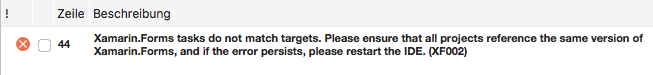
\includegraphics[width=1\textwidth]{images/Xamarin-Upgrade-Error.png}
		\caption{Fehlermeldung nach Aktualisierung aller Projektpakete}
		\label{fig:xamarinbuilderror}
	\end{figure}

	\newpage
	Der Einsatz von Webservices, siehe Abschnitt \ref{sec:mckbspecs}, ist einerseits auf die Deaktivierung des Xamarin Komponenten Store und andererseits auf die in Codeabschnitt \ref{lst:pluginerror} dargestellte Fehlermeldung bei hinzufügen des Plugins, \textbf{Xamarin.MySQL.Data.1.0.1} zurückzuführen.

	\begin{lstlisting}[caption={Fehlermeldung - Plugin Installation},label={lst:pluginerror},captionpos=b,style=SQL-Michalstyle]
Install failed. Rolling back...
Package 'Xamarin.MySql.Data.1.0.1' does not exist in project 'MCKB'
Package 'Xamarin.MySql.Data.1.0.1' does not exist in folder 
'/Users/maximilianpessl/Projects/MCKB/packages'
Executing nuget actions took 46,83 ms
Could not install package 'Xamarin.MySql.Data 1.0.1'. 
You are trying to install this package into a project that targets 
'.NETPortable,Version=v4.5,Profile=Profile7', 
but the package does not contain any assembly references or 
content files that are compatible with that framework. 
For more information, contact the package author.
	\end{lstlisting}

	Anpassungen an dem Projekt (MCKB PCL), zum Beispiel ändern der PCL Einstellungen welche in Zeile acht in Codeabschnitt \ref{lst:pluginerror} dargestellt sind, haben diese Fehlermeldung nicht beheben können, wodurch auf \textit{REST} als Webservice API zurückgegriffen werden musste. Das Plugin konnte den Projekten \textit{MCKB.Droid} und \textit{MCKB.iOS} hinzugefügt werden, jedoch bedeutete dies, dass die Client (Smartphone App) Server Kommunikation in beiden Projektordnern implementiert werden musste.

	Zur Messung der Kommunikationszeit zwischen dem Senden eines \textit{GET Request} und Empfangen einer \textit{Response} wurden vor dem Senden bzw. nach Empfangen die Systemzeit erhoben und in folgender Tabelle\ref{tab:clsvcom}\footnote{Xam.Forms.x - Xamarin.Forms.x App \\Xam.Nat.x - Xamarin.Native.x App \\Nat.Droid - Native Android\\ S - Send // R - Receive} festgehalten. Der dafür notwendige Code steht in Abschnitt \ref{chap:app} Codeabschnitt \ref{lst:measurecom} zur Verfügung.

	\begin{table}[h!]
		\centering
		\begin{tabular}{l|l|l|l|l|l|}
			\cline{2-6}
			                        & Xam.Forms.iOS    & Xam.Forms.Droid  & Xam.Nat.Droid& Xam.Nat.iOS  & Nat.Droid    \\ \hline
			\multicolumn{1}{|l|}{S} & 14:18:19.3465230 & 14:33:58.4397800 & 22:58:54.588 & 22:48:32.136 & 22:38:21.135 \\ \hline
			\multicolumn{1}{|l|}{R} & 14:18:19.8951310 & 14:34:01.3333110 & 22:58:54.717 & 22:48:32.260 & 22:38:37.775 \\ \hline
			\multicolumn{1}{|l|}{S} & 15:08:08.6368570 & 15:06:01.3397350 & - & - & - \\ \hline
			\multicolumn{1}{|l|}{R} & 15:08:09.3322090 & 15:06:03.1629580 & - & - & - \\ \hline
			\multicolumn{1}{|l|}{S} & 15:08:59.3353410 & 15:09:50.1086710 & - & - & - \\ \hline
			\multicolumn{1}{|l|}{R} & 15:08:59.8671340 & 15:09:51.9077950 & - & - & - \\ \hline
		\end{tabular}
		\label{tab:clsvcom}
		\caption{Ergebnisse der Kommunikationszeit über Webservice - Gegenüberstellung mit früheren Ergebnissen\cite{Maximilian2017} - Smartphone Simulatoren/Emulatoren}
	\end{table}
	
	
	\newpage
	Leider war es nicht möglich eine Messung für ein iOS und Android Smartphone durchzuführen, da es nicht möglich war die MCKB App auf einem iOS Gerät zu installieren. In Tabelle \ref{tab:clsvcomhard} sind daher nur die Ergebnisse der Android Version auf einem Alcatel Smartphone festgehalten.

	\begin{table}[h!]
		\centering
		\begin{tabular}{l|l|l|l|l|l|}
			\cline{2-6}
			                        & Xam.Forms.iOS    & Xam.Forms.Droid  & Xam.Nat.Droid& Xam.Nat.iOS  & Nat.Droid    \\ \hline
			\multicolumn{1}{|l|}{S} & 	  -			 & 14:32:04.8747300 & 		-	   & 	  -		  &  \\ \hline
			\multicolumn{1}{|l|}{R} & 	  -			 & 14:32:08.8170480 & 		-	   & 	  -		  &  \\ \hline
			\multicolumn{1}{|l|}{S} & 	  -			 & 15:12:15.8343150 & 		-	   & 	  -		  &  \\ \hline
			\multicolumn{1}{|l|}{R} & 	  -			 & 15:12:19.6612780 & 		-	   & 	  -		  &  \\ \hline
			\multicolumn{1}{|l|}{S} & 	  -			 & 15:13:21.6869140 & 		-	   & 	  -		  &  \\ \hline
			\multicolumn{1}{|l|}{R} & 	  -			 & 15:13:25.2504780 & 		-	   & 	  -		  &  \\ \hline
		\end{tabular}
		\label{tab:clsvcomhard}
		\caption{Ergebnisse der Kommunikationszeit über Webservice - Gegenüberstellung mit früheren Ergebnissen\cite{Maximilian2017} - Smartphone Hardware}
	\end{table}

	Eine Gegenüberstellung der Android App (STM32KB) mit dessen CP Versionen (STM32CP \& MCKB) war aufgrund der Änderungen seitens Microsoft nicht möglich. Da der Komponenten Store entfernt wurde kann die STM32CP App nicht mehr erstellt werden.

	Jedoch ist in beiden Tabellen erkennbar das es signifikante Unterschiede zwischen den CP Versionen der STM32KB App gab. Die Ladezeiten der Xamarin.Native App ist um einiges geringer als die der Xamarin.Forms Applikationen, wobei die Xamarin.Forms.iOS annähernd gleich schnell die Daten aus der Datenbank in die Applikation geladen hat.

	Die deutlich unterschiedlichen Ladezeiten für die Xamarin.Forms.Droid App könnten dadurch erklärt werden das ein Android Emulator nur die notwendigsten Systemprozesse im Hintergrund laufen lässt, während ein echtes Smartphone deutlich ausgelasteter ist.

	Bezüglich des Designs und der Programmierung der MCKB App bietet Xamarin.Forms eindeutig einen Zeitgewinn. Der Umstand bis zu 80 oder 90\% des Designs und der Geschäftslogik in dem PCL Projekt umzusetzen ist, sofern aufgrund der Spezifizierung möglich, genau das was CP-Developing so attraktiv macht. Allerdings gibt es eine Einschränkung bezüglich der MCKB.Droid App. In der Xamarin.Native Version gab es in der \textit{MainActivity} mehrere \textit{Fragments} um das Layout schnell wechseln zu können. Die Implementierung von Fragment ist im PCL Projekt nicht möglich. Weiters impliziert der Name Xamarin.Forms das es sich dabei um ein UI Framework mit klaren entscheidungsbasierten oder formularbasierten Abläufen in der App handelt. Erfordert eine CP App viele komplexe UI ELemente so empfiehlt es sich diese mit Xamarin.Native zu entwickeln. Da die MCKB App keine komplexen UI Elemente benötigt eignete sich Xamarin.Forms als Framework sehr gut.

	Das Design wird, wie Eingans erwähnt im PCL Projekt für iOS und Android gemeinsam in den jeweiligen \textit{XAML} Files erstellt. Zwar stellt Visual Studio for Mac eine Vorschau, für das Editieren von Design Files zur Verfügung, jedoch gab es hier immer wieder Probleme mit dem Rendern der UI Elemente. In Abbildung \ref{fig:mckbAppregister}\footnote{Der XAML Code befindet sich im Abschnitt \ref{chap:app} Codeabschnitt \ref{lst:mckbcodereg}} ist zur erkennen das man durch hinzufügen des \textit{BackgroundColor} Parameters die Ränder des Layout Elements darstellen kann um so die Grenzen eines \textit{StackLayout}, wie es die Page in Abbildung \ref{fig:mckbAppregister} verwendet, darzustellen.

	\begin{figure}[h!]
		\centering
		\begin{subfigure}
			\centering
			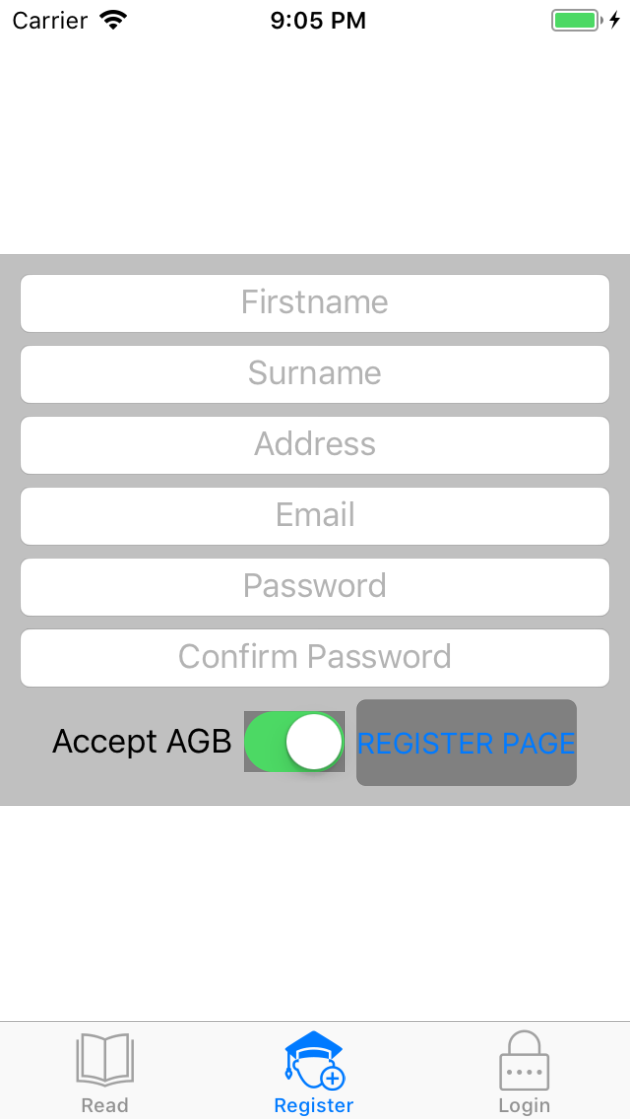
\includegraphics[width=.4\textwidth]{images/MCKB-iOS-Register-edit.png}
		\end{subfigure}
		\begin{subfigure}
			\centering
			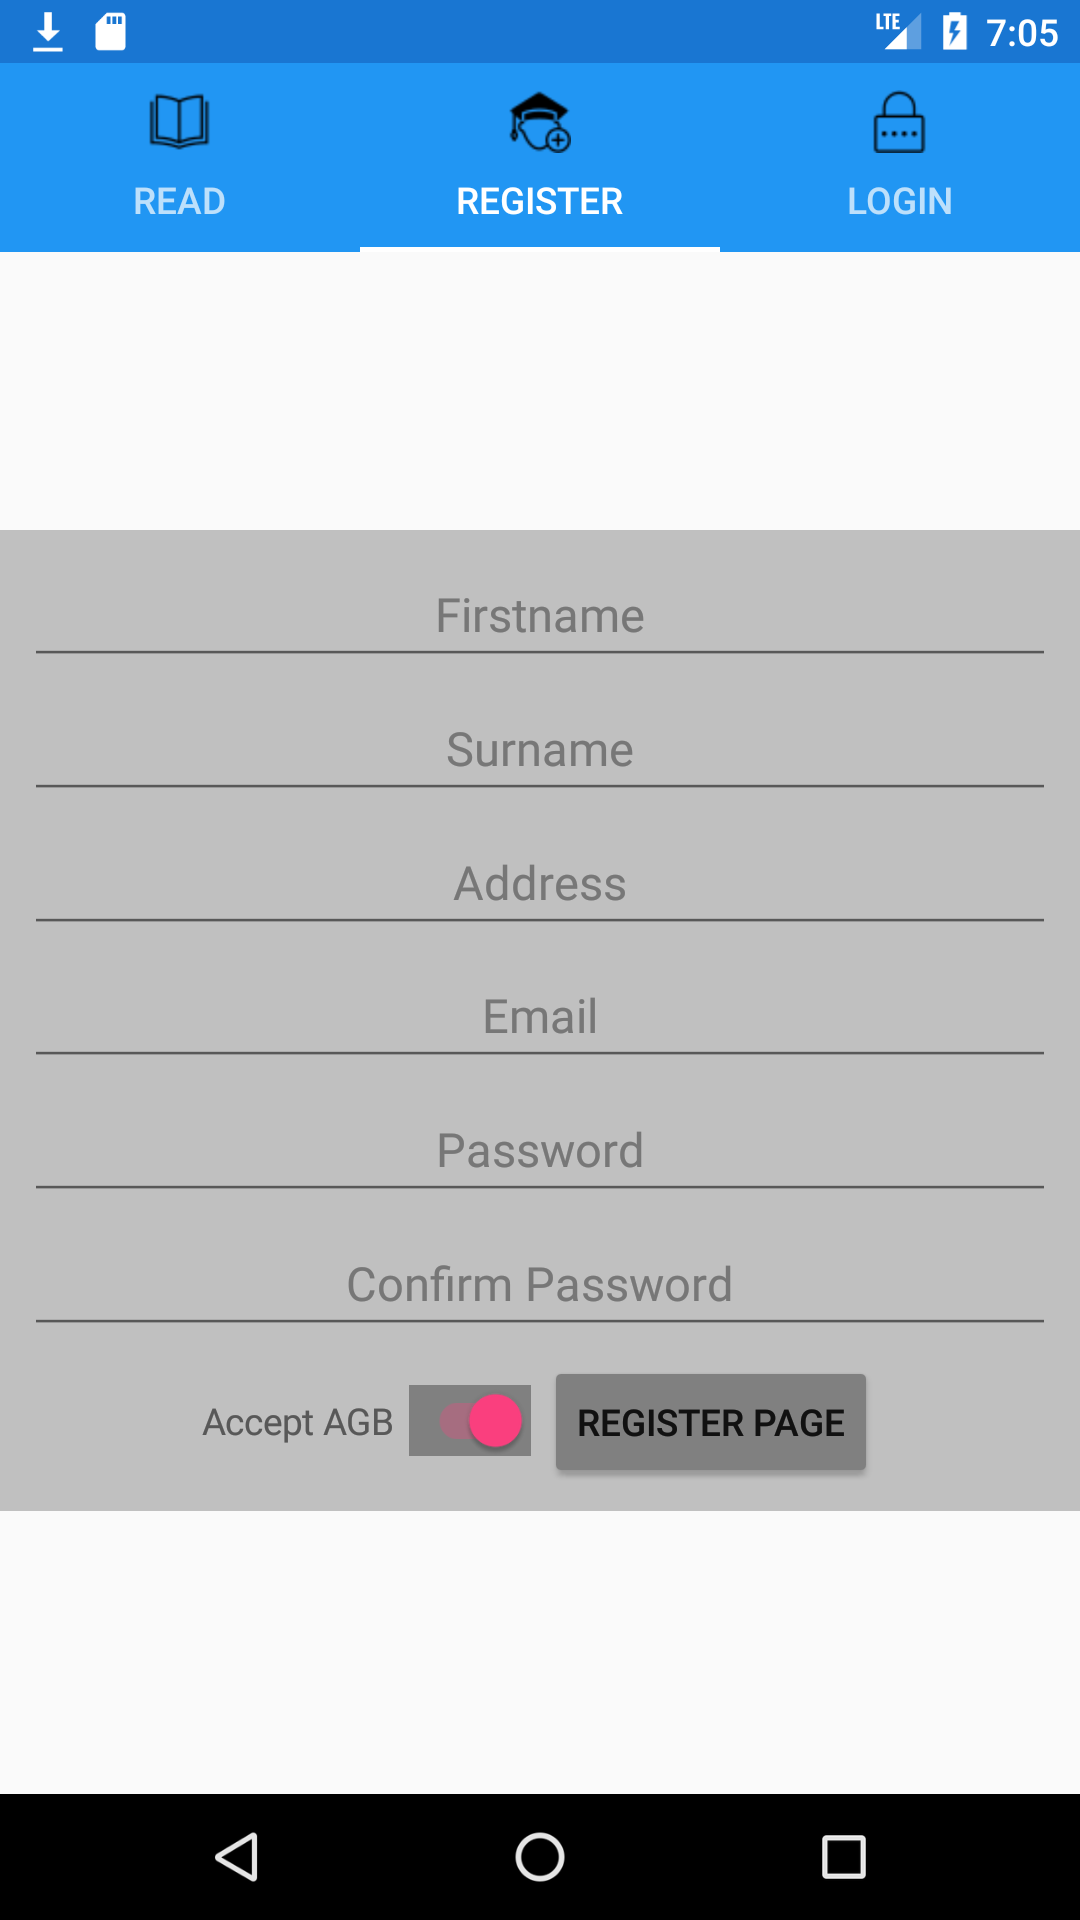
\includegraphics[width=.4\textwidth]{images/MCKB-Droid-Register-edit.png}
		\end{subfigure}
		\caption{Darstellen von Layout Grenzen}
		\label{fig:mckbAppregister}
	\end{figure}

	Selbiger Ansatz zur Abschätzung der Größe der UI Elemente wurde für die Login Page verwendet.

	In Kapitel \ref{chap:xamarinformsdevelopment} Abschnitt \ref{sec:mckspecs} ist die Spezifizierung für den \textit{UseCase - Artikel lesen} so definiert das durch eine Kategorie an Mikrocontroller die Artikel einer Kategorie durch Auswahl eines Dropdown angezeigt werden. Im Zuge der Programmierung wurde dies angepasst, ersichtlich in Abbildung \ref{fig:mckbApp}, da mit einer Liste an Kategorien die wiederum eine Liste an Artikeln enthält ein moderneres Design entworfen werden konnte.

	Das endgültige Design der MCKB Applikation ist in Kapitel \ref{chap:app} in Abbildung \ref{fig:mckbAppfinal} dargestellt. Der Code für dieses Design ist in Codeabschnitt \ref{lst:mckbdesigncode} zu finden. Plattformspezifische Design Parameter sind durch den \textbf{tag} \textit{$<$OnPlatform$><$/OnPlatform$>$} definiert. 




